\documentclass[12pt]{article}
\usepackage{geometry}
\geometry{a4paper, top=2cm, left=2cm, right=2cm, bottom=2cm}
\usepackage[utf8]{inputenc}
\usepackage{mathtools}
\usepackage{float}
\usepackage{amssymb}
\usepackage{mathrsfs}
\usepackage{qtree}[]
\usepackage{tabularx}
\usepackage{dsfont}
\usepackage{verbatim}

\usepackage{graphicx}


\usepackage{titlesec}


\titlelabel{\thetitle.\quad}
\usepackage{lscape}
\usepackage{indentfirst}

\usepackage{amsmath}
\usepackage{bm}

\newcommand*\rfrac[2]{{}^{#1}\!/_{#2}}

\DeclareMathOperator*{\argmin}{argmin}
\DeclareMathOperator*{\argmax}{argmax}


\newtagform{brackets}{[}{]}
\usetagform{brackets}

\usepackage{abstract}
\renewcommand{\abstractname}{}    % clear the title
\renewcommand{\absnamepos}{empty}

\usepackage{tikz}


\usepackage{blindtext}
\usepackage[flushleft]{threeparttable}

\usepackage{natbib}
\renewcommand{\bibsection}{}


\usepackage[labelfont={sc},labelsep=endash]{caption}
\captionsetup[table]{skip=1.5pt}
\captionsetup[figure]{skip=0pt}



\usepackage{fancyhdr}

%\pagestyle{fancy}
\fancyhf{}
%\rhead{\sc \monthyeardate\today}

\cfoot{ \thepage}

\renewcommand{\thesection}{\Roman{section}}
\renewcommand{\thesubsection}{\thesection.\Alph{subsection}}
\titleformat{\section}[hang]{\bfseries\fontfamily{phv}\selectfont}{\Roman{section}.}{4pt}{}[]
\titleformat{\subsection}[hang]{\scshape\itshape\fontfamily{ptm}\selectfont}{\thesection.\Alph{subsection}}{5pt}{}[]


\renewcommand{\baselinestretch}{1.1}
\usepackage{setspace}

\usepackage{times}

\usepackage{array}
\newcolumntype{L}[1]{>{\raggedright\let\newline\\\arraybackslash\hspace{0pt}}m{#1}}
\newcolumntype{C}[1]{>{\centering\let\newline\\\arraybackslash\hspace{0pt}}m{#1}}
\newcolumntype{R}[1]{>{\raggedleft\let\newline\\\arraybackslash\hspace{0pt}}m{#1}}


\newcommand\blfootnote[1]{%
  \begingroup
  \renewcommand\thefootnote{}\footnote{#1}%
  \addtocounter{footnote}{-1}%
  \endgroup
}

\usepackage[hang,flushmargin]{footmisc}
\usepackage{multirow}

\usepackage[nodayofweek]{datetime}
\newdateformat{mydate}{\twodigit{\THEDAY}{ }\shortmonthname[\THEMONTH], \THEYEAR}


\newcommand{\specialcell}[2][c]{%
  \begin{tabular}[#1]{@{}l@{}}#2\end{tabular}}

\fontfamily{lmss}\selectfont


%***citemodeis****
%*****************


\setlength{\parindent}{6mm}
\setlength{\parskip}{0em}

%\allsectionsfont{}
	

\begin{document}
	% line of code telling latex that your document is beginning


\vspace{2mm}
\begin{center}
\large\fontfamily{phv}\selectfont\bfseries\scshape{$\,\,\,\,$Results Report}
\end{center}
\vspace{5mm}

\noindent Clustering algorithm: {\bf\input{clalg.txt}} \\
\noindent Clustering 1st parameter: {\bf\input{clpar1.txt}} \\
\noindent Clustering 2nd parameter: {\bf\input{clpar2.txt}} \\ \\
\noindent Number of Clusters: {\bf\input{nuclust.txt}} \\ \\
\noindent Bandwidth: {\bf\input{bw.txt}m} \\
\noindent minimum percentage RDP built in mode year : {\bf\input{tr1.txt}} \\
\noindent minimum percentage RDP built in $\pm$ 1 mode year : {\bf\input{tr2.txt}} \\
\noindent minimum percentage RDP built in mode year : {\bf\input{tr1.txt}} \\
\noindent time window around mode year : {\bf$\pm$\input{tw.txt} years} \\ 

\begin{figure}[H]
\centering
\begin{minipage}{.5\textwidth}
  \centering
  \includegraphics[width=\linewidth]{transperclust.pdf}
\end{minipage}%
\begin{minipage}{.5\textwidth}
  \centering
  \includegraphics[width=\linewidth]{rdpperclust.pdf}
\end{minipage}
\end{figure}

\begin{figure}[H]
\centering
\begin{minipage}{.5\textwidth}
  \centering
  \includegraphics[width=\linewidth]{gisthist.pdf}
\end{minipage}%
\begin{minipage}{.5\textwidth}
  \centering
  \includegraphics[width=\linewidth]{gisthistprepo.pdf}
\end{minipage}
\end{figure}

\begin{table}[H]
\centering
1                   &      599.67&            \\
2                   &    101.1361&            \\
Total               &    366.3724&            \\

\end{table}



\pagebreak

\noindent {\bf Raw log-price means. } \\
\noindent pre (post) is one year before (after) mode year.
\begin{figure}[H]
\centering
\includegraphics[width=.9\linewidth]{raw_plot1.pdf}
\end{figure}

\noindent {\bf Adjusted log-price means. Year$\times$municipality, month, and cluster FE.}\\ 
\noindent pre (post) is one year before (after) mode year.
\begin{figure}[H]
\centering
\includegraphics[width=.9\linewidth]{reg_plot1.pdf}
\end{figure}

\pagebreak

\noindent {\bf Clusters }
\begin{figure}[H]
\centering
\includegraphics[width=.8\linewidth]{plot.pdf}
\end{figure}

\noindent {\bf Clusters (zoomed in).}
\begin{figure}[H]
\centering
\includegraphics[width=.8\linewidth]{plotzoom.pdf}
\end{figure}

\pagebreak
{ \small
\noindent {\bf Raw price means}, pre (post) is one year before (after) mode year.
\begin{figure}[H]
\centering
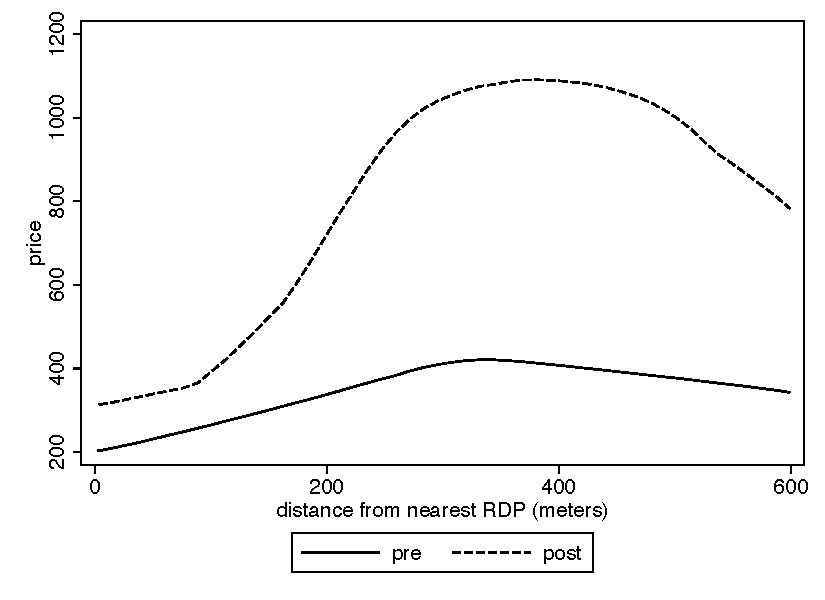
\includegraphics[width=.54\linewidth]{raw_plot2.pdf}
\end{figure}

\noindent {\bf Raw log-price means}, pre (post) is {\bf two} before (after) mode year.
\begin{figure}[H]
\centering
\includegraphics[width=.54\linewidth]{raw_plot3.pdf}
\end{figure}

\noindent {\bf Raw price means}, pre (post) is {\bf two}  year before (after) mode year.
\begin{figure}[H]
\centering
\includegraphics[width=.54\linewidth]{raw_plot4.pdf}
\end{figure}
}

\pagebreak
{ \small
\noindent {\bf reg-adjusted log-price}, no cluster FE.
\begin{figure}[H]
\centering
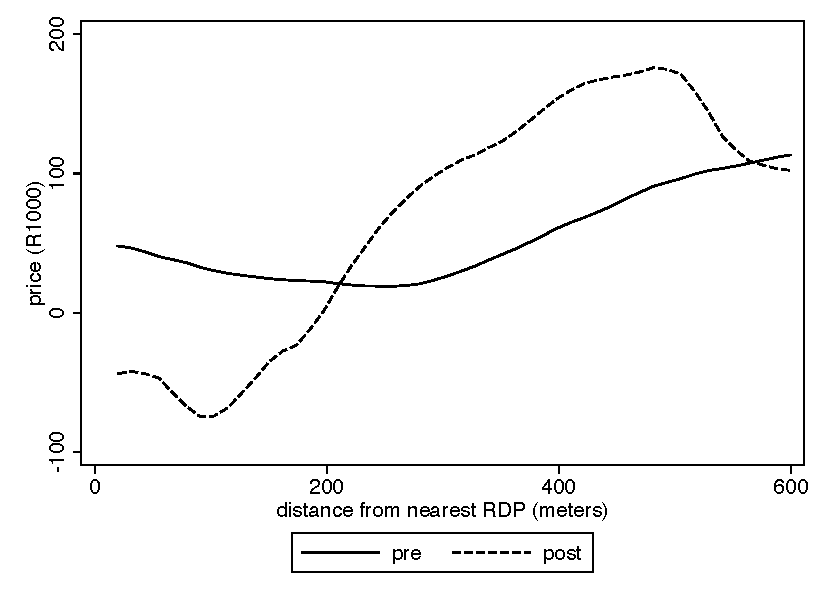
\includegraphics[width=.54\linewidth]{reg_plot2.pdf}
\end{figure}

\noindent {\bf reg-adjusted log-price}, $\pm$ 2 years.
\begin{figure}[H]
\centering
\includegraphics[width=.54\linewidth]{reg_plot3.pdf}
\end{figure}

\noindent {\bf reg-adjusted log-price}, $\pm$ 2 years, no cluster FE.
\begin{figure}[H]
\centering
\includegraphics[width=.54\linewidth]{reg_plot4.pdf}
\end{figure}
}


\end{document}












